% Yolymatics Tutorials — Linear Transformations Slides
% Build with: pdflatex -interaction=nonstopmode -halt-on-error linear_transformations_slides.tex

\documentclass[aspectratio=169,professionalfonts]{beamer}

% Core packages
\usepackage[T1]{fontenc}
\usepackage[utf8]{inputenc}
\usepackage{lmodern}
\usepackage{amsmath, amssymb}
\usepackage{graphicx}
\usepackage{booktabs}
\usepackage{microtype}
\usepackage{tikz}
\usetikzlibrary{positioning,calc,shapes,arrows.meta,decorations.pathreplacing}
\usepackage{hyperref}

% Professional brand colors - elegant and modern
\definecolor{YolyPrimary}{HTML}{1E3A8A}   % deep professional blue
\definecolor{YolyAccent}{HTML}{F59E0B}    % warm amber
\definecolor{YolyDark}{HTML}{0F172A}      % slate dark
\definecolor{YolyLight}{HTML}{F8FAFC}     % very light gray
\definecolor{YolyMid}{HTML}{475569}       % mid slate
\definecolor{YolySecondary}{HTML}{3B82F6} % bright blue

% Beamer theme and professional styling
\mode<presentation>{
  \usetheme{Madrid}
  \usecolortheme{default}
  \setbeamertemplate{navigation symbols}{}
  
  % Main structure colors
  \setbeamercolor{structure}{fg=YolyPrimary}
  \setbeamercolor{title}{fg=white,bg=YolyPrimary}
  \setbeamercolor{frametitle}{fg=YolyDark,bg=YolyLight}
  
  % Block styling - more elegant
  \setbeamercolor{block title}{fg=white,bg=YolyPrimary}
  \setbeamercolor{block body}{fg=YolyDark,bg=YolyLight}
  \setbeamercolor{block title example}{fg=white,bg=YolyAccent}
  \setbeamercolor{block body example}{fg=YolyDark,bg=YolyLight}
  
  % Item colors
  \setbeamercolor{itemize item}{fg=YolyAccent}
  \setbeamercolor{itemize subitem}{fg=YolySecondary}
  \setbeamercolor{enumerate item}{fg=YolyAccent}
  
  % Alert color
  \setbeamercolor{alerted text}{fg=YolyAccent}
  
  % Frame title template with underline
  \setbeamertemplate{frametitle}{
    \vspace{0.3cm}
    \begin{beamercolorbox}[wd=\paperwidth,ht=1.2cm,dp=0.3cm,leftskip=0.5cm]{frametitle}
      \usebeamerfont{frametitle}\insertframetitle
      \ifx\insertframesubtitle\@empty
      \else
        \\{\small\usebeamerfont{framesubtitle}\insertframesubtitle}
      \fi
    \end{beamercolorbox}
    \vspace{-0.15cm}
    \textcolor{YolyAccent}{\rule{\paperwidth}{2pt}}
  }
  
  % Rounded blocks
  \setbeamertemplate{blocks}[rounded][shadow=false]
}

% Custom footline with brand + contact + slide count - more elegant
\setbeamertemplate{footline}{%
  \leavevmode
  \hbox{%
  \begin{beamercolorbox}[wd=.33\paperwidth,ht=2.8ex,dp=1.2ex,left]{frametitle}%
    \hspace*{1.5ex}\textbf{\textcolor{YolyPrimary}{Yolymatics Tutorials}}
  \end{beamercolorbox}%
  \begin{beamercolorbox}[wd=.34\paperwidth,ht=2.8ex,dp=1.2ex,center]{frametitle}%
    \textcolor{YolyMid}{\href{mailto:yolymatics007@gmail.com}{yolymatics007@gmail.com}}
  \end{beamercolorbox}%
  \begin{beamercolorbox}[wd=.33\paperwidth,ht=2.8ex,dp=1.2ex,right]{frametitle}%
    \textcolor{YolyMid}{\insertframenumber{} / \inserttotalframenumber}\hspace*{1.5ex}
  \end{beamercolorbox}}
  \vskip0pt}

% Professional section title page with geometric design
\AtBeginSection[]{
  \begin{frame}[plain,noframenumbering]
    \vfill
    \begin{tikzpicture}[remember picture,overlay]
      % Background accent
      \fill[YolyPrimary!10] (current page.north west) rectangle (current page.south east);
      % Geometric accent bars
      \fill[YolyPrimary] (current page.north west) rectangle ($(current page.north east)+(0,-0.5cm)$);
      \fill[YolyAccent] (current page.north west) rectangle ($(current page.north east)+(0,-0.3cm)$);
    \end{tikzpicture}
    \vspace*{4cm}
    \begin{center}
      {\usebeamerfont{title}\textcolor{YolyPrimary}{\LARGE\insertsection}}
      \vspace{0.5cm}
      
      \textcolor{YolyAccent}{\rule{0.6\linewidth}{3pt}}
    \end{center}
    \vfill
  \end{frame}}

% Title metadata
\title{Linear Transformations}
\subtitle{Geometric Transformations in the Plane}
\author{Yolymatics Tutorials}
\institute{\href{mailto:yolymatics007@gmail.com}{yolymatics007@gmail.com}}
\date{\today}

% Modern professional title background with geometric design
\setbeamertemplate{title page}{%
  \begin{tikzpicture}[remember picture,overlay]
    % Main blue background
    \fill[YolyPrimary] (current page.north west) rectangle ($(current page.north east)+(0,-5cm)$);
    % Accent stripe - amber
    \fill[YolyAccent] ($(current page.north west)+(0,-5cm)$) rectangle ($(current page.north east)+(0,-5.4cm)$);
    % Light background for lower section
    \fill[YolyLight] ($(current page.north west)+(0,-5.4cm)$) rectangle (current page.south east);
    
    % Geometric decorative elements
    \fill[YolySecondary,opacity=0.3] (current page.north east) circle (3cm);
    \fill[YolyAccent,opacity=0.2] ($(current page.north west)+(2cm,-2cm)$) circle (2cm);
  \end{tikzpicture}%
  
  \vspace*{2.5cm}
  \begin{flushleft}
    \hspace{0.8cm}
    {\color{white}\fontsize{32}{36}\selectfont\textbf{\inserttitle}}
    \par\vspace{0.4cm}
    \hspace{0.8cm}
    {\color{YolyLight}\Large\insertsubtitle}
  \end{flushleft}
  
  \vfill
  
  \begin{flushleft}
    \hspace{0.8cm}
    \textcolor{YolyDark}{\Large\textbf{\insertauthor}}\\[0.3ex]
    \hspace{0.8cm}
    \textcolor{YolyMid}{\large\insertinstitute}
  \end{flushleft}
  \vspace*{1cm}
}

% Convenience
\newcommand{\R}{\mathbb{R}}
\newcommand{\vect}[1]{\mathbf{#1}}
\DeclareMathOperator{\proj}{proj}

\begin{document}

\begin{frame}[plain]
  \titlepage
\end{frame}

\begin{frame}{Today's objectives}
  \begin{itemize}
    \item Understand what linear transformations are and their properties
    \item Learn the five fundamental transformations: scaling, reflection, projection, shearing, rotation
    \item Represent transformations using matrices
    \item Compose transformations and understand geometric effects
    \item Apply transformations to solve geometric problems
  \end{itemize}
\end{frame}

\section{Foundations}

\begin{frame}{What is a transformation?}
  \begin{block}{Definition}
    A \textbf{transformation} $T: \R^2 \to \R^2$ is a function that takes points (vectors) in the plane and maps them to other points in the plane.
    
    \vspace{0.5em}
    If $\vect{v} = \begin{bmatrix} x \\ y \end{bmatrix}$, then $T(\vect{v}) = \begin{bmatrix} x' \\ y' \end{bmatrix}$ is the \textbf{image} of $\vect{v}$ under $T$.
  \end{block}
  
  \vspace{1em}
  \textbf{Notation:}
  \begin{itemize}
    \item $T(\vect{v})$ or $T\vect{v}$ = image of vector $\vect{v}$
    \item Original object = \textbf{pre-image}
    \item Transformed object = \textbf{image}
  \end{itemize}
\end{frame}

\begin{frame}{Linear transformations: Definition}
  \begin{block}{Definition}
    A transformation $T: \R^2 \to \R^2$ is \textbf{linear} if it satisfies two properties:
    
    \vspace{0.5em}
    \textbf{1. Additivity:} $T(\vect{u} + \vect{v}) = T(\vect{u}) + T(\vect{v})$ for all vectors $\vect{u}, \vect{v}$
    
    \textbf{2. Homogeneity:} $T(c\vect{v}) = cT(\vect{v})$ for all scalars $c$ and vectors $\vect{v}$
  \end{block}
  
  \vspace{1em}
  \begin{alertblock}{Key consequence}
    Every linear transformation can be represented by a matrix: $T(\vect{v}) = A\vect{v}$
  \end{alertblock}
  
  \vspace{0.5em}
  \textbf{Important:} Linear transformations always map the origin to itself: $T(\vect{0}) = \vect{0}$
\end{frame}

\begin{frame}{Matrix representation}
  \begin{block}{How to find the matrix}
    To find the matrix $A$ for a linear transformation $T$:
    
    \vspace{0.5em}
    \textbf{Step 1:} Find where $T$ sends the standard basis vectors:
    \[
    \vect{e}_1 = \begin{bmatrix} 1 \\ 0 \end{bmatrix}, \quad \vect{e}_2 = \begin{bmatrix} 0 \\ 1 \end{bmatrix}
    \]
    
    \textbf{Step 2:} The matrix $A$ has these images as its columns:
    \[
    A = \begin{bmatrix} | & | \\ T(\vect{e}_1) & T(\vect{e}_2) \\ | & | \end{bmatrix}
    \]
  \end{block}
  
  \vspace{0.5em}
  Then for any vector $\vect{v}$: 
  \[
  T(\vect{v}) = A\vect{v}
  \]
\end{frame}

\begin{frame}{Properties of linear transformations}
  \begin{columns}[T]
    \begin{column}{0.48\textwidth}
      \textbf{Linear transformations preserve:}
      \begin{itemize}
        \item The origin
        \item Straight lines
        \item Parallelism
        \item Ratios of distances along lines
      \end{itemize}
    \end{column}
    \begin{column}{0.48\textwidth}
      \textbf{They may change:}
      \begin{itemize}
        \item Lengths
        \item Angles
        \item Areas
        \item Orientation
      \end{itemize}
    \end{column}
  \end{columns}
  
  \vspace{1.5em}
  \begin{exampleblock}{Non-examples}
    These are NOT linear transformations:
    \begin{itemize}
      \item Translation: $(x,y) \mapsto (x+3, y+2)$ — doesn't fix origin
      \item $(x,y) \mapsto (x^2, y)$ — doesn't preserve additivity
    \end{itemize}
  \end{exampleblock}
\end{frame}

\section{Scaling}

\begin{frame}{Scaling transformations}
  \begin{block}{Definition}
    A \textbf{scaling} (or dilation) multiplies coordinates by constants:
    \[
    T(x,y) = (kx, ly)
    \]
    where $k, l \in \R$ are the scaling factors.
  \end{block}
  
  \begin{columns}[T]
    \begin{column}{0.48\textwidth}
      \textbf{Matrix form:}
      \[
      A = \begin{bmatrix} k & 0 \\ 0 & l \end{bmatrix}
      \]
      
      \vspace{1em}
      \textbf{Special cases:}
      \begin{itemize}
        \item $k = l$: uniform scaling
        \item $k = l = 1$: identity
        \item $k = l = -1$: point reflection through origin
      \end{itemize}
    \end{column}
    \begin{column}{0.48\textwidth}
      \centering
      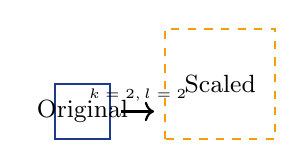
\begin{tikzpicture}[scale=0.7]
        % Original square
        \draw[thick,YolyPrimary] (0,0) rectangle (1,1);
        \node at (0.5,0.5) {\small Original};
        
        % Scaled square
        \draw[thick,YolyAccent,dashed] (2,0) rectangle (4,2);
        \node at (3,1) {\small Scaled};
        
        % Arrow
        \draw[->,thick] (1.2,0.5) -- (1.8,0.5);
        \node[above] at (1.5,0.5) {\tiny $k=2, l=2$};
      \end{tikzpicture}
    \end{column}
  \end{columns}
\end{frame}

\begin{frame}{Scaling: Examples and effects}
  \begin{exampleblock}{Example: Stretch and compress}
    Matrix $A = \begin{bmatrix} 3 & 0 \\ 0 & 0.5 \end{bmatrix}$
    \begin{itemize}
      \item Stretches by factor 3 in $x$-direction
      \item Compresses by factor 0.5 in $y$-direction
    \end{itemize}
  \end{exampleblock}
  
  \vspace{1em}
  \textbf{Geometric effects:}
  \begin{itemize}
    \item If $|k| > 1$: stretch in $x$-direction
    \item If $0 < |k| < 1$: compress in $x$-direction
    \item If $k < 0$: also reflects across $y$-axis
    \item Area multiplied by $|kl|$
  \end{itemize}
\end{frame}

\section{Reflections}

\begin{frame}{Reflection transformations}
  \begin{block}{Common reflections}
    \textbf{Across $x$-axis:} $(x,y) \mapsto (x,-y)$ \quad Matrix: $\begin{bmatrix} 1 & 0 \\ 0 & -1 \end{bmatrix}$
    
    \vspace{0.5em}
    \textbf{Across $y$-axis:} $(x,y) \mapsto (-x,y)$ \quad Matrix: $\begin{bmatrix} -1 & 0 \\ 0 & 1 \end{bmatrix}$
    
    \vspace{0.5em}
    \textbf{Across line $y=x$:} $(x,y) \mapsto (y,x)$ \quad Matrix: $\begin{bmatrix} 0 & 1 \\ 1 & 0 \end{bmatrix}$
    
    \vspace{0.5em}
    \textbf{Across line $y=-x$:} $(x,y) \mapsto (-y,-x)$ \quad Matrix: $\begin{bmatrix} 0 & -1 \\ -1 & 0 \end{bmatrix}$
  \end{block}
  
  \vspace{0.5em}
  \textbf{Properties:}
  \begin{itemize}
    \item Reflections preserve distances and angles
    \item Applying same reflection twice gives identity: $R \circ R = I$
    \item Determinant = $-1$ (reverses orientation)
  \end{itemize}
\end{frame}

\begin{frame}{Reflection across arbitrary lines}
  \begin{block}{Reflection across line through origin at angle $\theta$}
    The matrix for reflection across a line making angle $\theta$ with the positive $x$-axis:
    \[
    R_\theta = \begin{bmatrix} \cos(2\theta) & \sin(2\theta) \\ \sin(2\theta) & -\cos(2\theta) \end{bmatrix}
    \]
  \end{block}
  
  \vspace{1em}
  \begin{exampleblock}{Verification for common cases}
    \begin{itemize}
      \item $\theta = 0$ ($x$-axis): $R_0 = \begin{bmatrix} 1 & 0 \\ 0 & -1 \end{bmatrix}$ \checkmark
      \item $\theta = \pi/4$ (line $y=x$): $R_{\pi/4} = \begin{bmatrix} 0 & 1 \\ 1 & 0 \end{bmatrix}$ \checkmark
    \end{itemize}
  \end{exampleblock}
\end{frame}

\section{Projections}

\begin{frame}{Projection transformations}
  \begin{block}{Definition}
    A \textbf{projection} maps points onto a line or subspace, collapsing one dimension.
  \end{block}
  
  \begin{columns}[T]
    \begin{column}{0.48\textwidth}
      \textbf{Common projections:}
      
      \vspace{0.5em}
      \textbf{Onto $x$-axis:} 
      \[
      (x,y) \mapsto (x,0)
      \]
      \[
      P_x = \begin{bmatrix} 1 & 0 \\ 0 & 0 \end{bmatrix}
      \]
      
      \vspace{0.5em}
      \textbf{Onto $y$-axis:} 
      \[
      (x,y) \mapsto (0,y)
      \]
      \[
      P_y = \begin{bmatrix} 0 & 0 \\ 0 & 1 \end{bmatrix}
      \]
    \end{column}
    \begin{column}{0.48\textwidth}
      \centering
      \begin{tikzpicture}[scale=0.8]
        % Axes
        \draw[->] (-0.5,0) -- (3,0) node[right] {$x$};
        \draw[->] (0,-0.5) -- (0,2.5) node[above] {$y$};
        
        % Original point
        \fill[YolyPrimary] (2,2) circle (2pt);
        \node[above right] at (2,2) {$(x,y)$};
        
        % Projection
        \fill[YolyAccent] (2,0) circle (2pt);
        \node[below] at (2,0) {$(x,0)$};
        
        % Dashed line
        \draw[dashed,YolyMid] (2,2) -- (2,0);
      \end{tikzpicture}
      
      \vspace{0.3em}
      {\small Projection onto $x$-axis}
    \end{column}
  \end{columns}
  
  \vspace{0.5em}
  \textbf{Key property:} $P \circ P = P$ (applying twice = applying once)
\end{frame}

\begin{frame}{Projection onto arbitrary lines}
  \begin{block}{Projection onto line through origin}
    For a unit vector $\vect{u} = \begin{bmatrix} \cos\theta \\ \sin\theta \end{bmatrix}$ along a line:
    
    \vspace{0.5em}
    The projection matrix is:
    \[
    P = \vect{u}\vect{u}^T = \begin{bmatrix} \cos^2\theta & \cos\theta\sin\theta \\ \cos\theta\sin\theta & \sin^2\theta \end{bmatrix}
    \]
  \end{block}
  
  \vspace{1em}
  \textbf{Geometric interpretation:}
  \begin{itemize}
    \item Projects every point perpendicularly onto the line
    \item Points on the line stay fixed
    \item Points perpendicular to the line map to origin
  \end{itemize}
\end{frame}

\section{Shearing}

\begin{frame}{Shear transformations}
  \begin{block}{Definition}
    A \textbf{shear} "slides" one coordinate direction by an amount proportional to the other.
  \end{block}
  
  \begin{columns}[T]
    \begin{column}{0.48\textwidth}
      \textbf{Horizontal shear:}
      \[
      T(x,y) = (x + ky, y)
      \]
      \[
      S_x = \begin{bmatrix} 1 & k \\ 0 & 1 \end{bmatrix}
      \]
      
      \vspace{1em}
      \textbf{Vertical shear:}
      \[
      T(x,y) = (x, kx + y)
      \]
      \[
      S_y = \begin{bmatrix} 1 & 0 \\ k & 1 \end{bmatrix}
      \]
    \end{column}
    \begin{column}{0.48\textwidth}
      \centering
      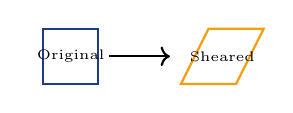
\begin{tikzpicture}[scale=0.7]
        % Original square
        \draw[thick,YolyPrimary] (0,0) rectangle (1,1);
        \node at (0.5,0.5) {\tiny Original};
        
        % Sheared parallelogram
        \draw[thick,YolyAccent] (2.5,0) -- (3.5,0) -- (4,1) -- (3,1) -- cycle;
        \node at (3.25,0.5) {\tiny Sheared};
        
        % Arrow
        \draw[->,thick] (1.2,0.5) -- (2.3,0.5);
      \end{tikzpicture}
      
      \vspace{0.5em}
      {\small Horizontal shear with $k=0.5$}
    \end{column}
  \end{columns}
  
  \vspace{1em}
  \textbf{Properties:}
  \begin{itemize}
    \item Preserves areas (determinant = 1)
    \item One axis stays fixed
    \item Creates "slanting" or "skewing" effect
  \end{itemize}
\end{frame}

\section{Rotation}

\begin{frame}{Rotation transformations}
  \begin{block}{Rotation by angle $\theta$ counterclockwise}
    \[
    R_\theta = \begin{bmatrix} \cos\theta & -\sin\theta \\ \sin\theta & \cos\theta \end{bmatrix}
    \]
    
    \vspace{0.5em}
    This rotates every point by angle $\theta$ counterclockwise around the origin.
  \end{block}
  
  \begin{columns}[T]
    \begin{column}{0.48\textwidth}
      \textbf{Common angles:}
      \begin{itemize}
        \item $90^\circ$: $\begin{bmatrix} 0 & -1 \\ 1 & 0 \end{bmatrix}$
        \item $180^\circ$: $\begin{bmatrix} -1 & 0 \\ 0 & -1 \end{bmatrix}$
        \item $270^\circ$: $\begin{bmatrix} 0 & 1 \\ -1 & 0 \end{bmatrix}$
      \end{itemize}
    \end{column}
    \begin{column}{0.48\textwidth}
      \textbf{Properties:}
      \begin{itemize}
        \item Preserves distances
        \item Preserves angles
        \item Determinant = 1
        \item $R_{-\theta} = R_\theta^{-1} = R_\theta^T$
      \end{itemize}
    \end{column}
  \end{columns}
\end{frame}

\begin{frame}{Composing transformations}
  \begin{block}{Composition}
    To apply transformation $T_2$ after $T_1$: $(T_2 \circ T_1)(\vect{v}) = T_2(T_1(\vect{v}))$
    
    \vspace{0.5em}
    If $T_1$ has matrix $A_1$ and $T_2$ has matrix $A_2$, then:
    \[
    T_2 \circ T_1 \text{ has matrix } A_2 A_1 \quad \text{(note the order!)}
    \]
  \end{block}
  
  \vspace{1em}
  \begin{alertblock}{Important}
    Matrix multiplication is NOT commutative: $A_2A_1 \neq A_1A_2$ in general.
    
    Order matters! "Rotate then scale" $\neq$ "Scale then rotate"
  \end{alertblock}
\end{frame}

\begin{frame}{Working with transformations: A procedure}
  \begin{block}{Step-by-step guide}
    \textbf{To find the effect of transformation $T$:}
    
    \begin{enumerate}
      \item \textbf{Find the matrix:} Determine $T(\vect{e}_1)$ and $T(\vect{e}_2)$, or use known forms
      \item \textbf{Apply to point:} Compute $A\vect{v}$ using matrix multiplication
      \item \textbf{Geometric interpretation:} Describe the effect (rotation? stretch? etc.)
    \end{enumerate}
    
    \vspace{0.5em}
    \textbf{To compose transformations:}
    \begin{enumerate}
      \item Find matrix for each transformation
      \item Multiply matrices in reverse order: $A_2A_1$ for "$T_1$ then $T_2$"
      \item Apply the composite matrix
    \end{enumerate}
  \end{block}
\end{frame}

\section{Determining Transformation Matrices}

\begin{frame}{How to find transformation matrices}
  \begin{block}{Method 1: Using standard basis vectors}
    For a transformation $T: \mathbb{R}^2 \to \mathbb{R}^2$:
    
    \vspace{0.5em}
    \textbf{Step 1:} Find where the standard basis vectors map:
    \begin{itemize}
      \item $\vect{e}_1 = \begin{bmatrix} 1 \\ 0 \end{bmatrix} \mapsto T(\vect{e}_1) = \begin{bmatrix} a \\ c \end{bmatrix}$
      \item $\vect{e}_2 = \begin{bmatrix} 0 \\ 1 \end{bmatrix} \mapsto T(\vect{e}_2) = \begin{bmatrix} b \\ d \end{bmatrix}$
    \end{itemize}
    
    \textbf{Step 2:} The matrix is:
    \[
    A = \begin{bmatrix} a & b \\ c & d \end{bmatrix}
    \]
  \end{block}
  
  \vspace{0.5em}
  \textbf{Why?} Because $T(\vect{v}) = A\vect{v}$ for all $\vect{v}$
\end{frame}

\begin{frame}{Determining matrices: Example 1}
  \begin{exampleblock}{Example: Reflection across line $y = x$}
    Find the matrix for reflection across the line $y = x$.
    
    \vspace{0.5em}
    \textbf{Solution:}
    \begin{itemize}
      \item The point $(1, 0)$ reflects to $(0, 1)$: 
      $T(\vect{e}_1) = \begin{bmatrix} 0 \\ 1 \end{bmatrix}$
      
      \item The point $(0, 1)$ reflects to $(1, 0)$: 
      $T(\vect{e}_2) = \begin{bmatrix} 1 \\ 0 \end{bmatrix}$
    \end{itemize}
    
    Therefore: $A = \begin{bmatrix} 0 & 1 \\ 1 & 0 \end{bmatrix}$
  \end{exampleblock}
  
  \vspace{0.5em}
  \textbf{Verify:} $(x, y) \mapsto (y, x)$ \checkmark
\end{frame}

\begin{frame}{Determining matrices: Example 2}
  \begin{exampleblock}{Example: Projection onto $x$-axis}
    Find the matrix for projection onto the $x$-axis.
    
    \vspace{0.5em}
    \textbf{Solution:}
    \begin{itemize}
      \item $(1, 0)$ projects to $(1, 0)$: 
      $T(\vect{e}_1) = \begin{bmatrix} 1 \\ 0 \end{bmatrix}$
      
      \item $(0, 1)$ projects to $(0, 0)$: 
      $T(\vect{e}_2) = \begin{bmatrix} 0 \\ 0 \end{bmatrix}$
    \end{itemize}
    
    Therefore: $A = \begin{bmatrix} 1 & 0 \\ 0 & 0 \end{bmatrix}$
  \end{exampleblock}
  
  \vspace{0.5em}
  \textbf{Verify:} $(x, y) \mapsto (x, 0)$ \checkmark
\end{frame}

\begin{frame}{Method 2: Using geometric properties}
  \begin{block}{For rotations}
    Rotation by angle $\theta$ counterclockwise about the origin:
    \[
    R_\theta = \begin{bmatrix} \cos\theta & -\sin\theta \\ \sin\theta & \cos\theta \end{bmatrix}
    \]
  \end{block}
  
  \begin{block}{For reflections across a line through origin}
    Reflection across line making angle $\theta$ with $x$-axis:
    \[
    \text{Refl}_\theta = \begin{bmatrix} \cos(2\theta) & \sin(2\theta) \\ \sin(2\theta) & -\cos(2\theta) \end{bmatrix}
    \]
  \end{block}
  
  \vspace{0.5em}
  \textbf{Tip:} Memorize these formulas or derive from basis vectors!
\end{frame}

\section{Transformation of Lines and Planes}

\begin{frame}{How lines transform}
  \begin{block}{Key principle}
    Linear transformations map lines to lines (or points).
    
    \vspace{0.5em}
    To find the image of a line $L$ under transformation $T$:
  \end{block}
  
  \begin{enumerate}
    \item \textbf{Parametric method:}
    \begin{itemize}
      \item Write line in parametric form: $\vect{r}(t) = \vect{a} + t\vect{d}$
      \item Apply transformation: $T(\vect{r}(t)) = T(\vect{a}) + tT(\vect{d})$
      \item This gives the image line
    \end{itemize}
    
    \item \textbf{Two-point method:}
    \begin{itemize}
      \item Find two points on the line
      \item Transform both points
      \item Image line passes through these two image points
    \end{itemize}
  \end{enumerate}
\end{frame}

\begin{frame}{Transforming lines: Example}
  \begin{exampleblock}{Example}
    Let $A = \begin{bmatrix} 2 & 0 \\ 0 & 3 \end{bmatrix}$ (scaling). 
    Find the image of the line $y = 2x + 1$.
    
    \vspace{0.5em}
    \textbf{Solution using two points:}
    \begin{itemize}
      \item Point 1: $(0, 1)$ maps to $A\begin{bmatrix} 0 \\ 1 \end{bmatrix} = \begin{bmatrix} 0 \\ 3 \end{bmatrix}$
      
      \item Point 2: $(1, 3)$ maps to $A\begin{bmatrix} 1 \\ 3 \end{bmatrix} = \begin{bmatrix} 2 \\ 9 \end{bmatrix}$
    \end{itemize}
    
    Slope of image line: $\frac{9-3}{2-0} = 3$
    
    Equation: $y - 3 = 3(x - 0)$ gives $y = 3x + 3$
  \end{exampleblock}
\end{frame}

\begin{frame}{Transforming lines: Parametric approach}
  \begin{exampleblock}{Same example using parametric form}
    Line $y = 2x + 1$ in parametric form:
    \[
    \vect{r}(t) = \begin{bmatrix} 0 \\ 1 \end{bmatrix} + t\begin{bmatrix} 1 \\ 2 \end{bmatrix}
    \]
    
    Apply $A = \begin{bmatrix} 2 & 0 \\ 0 & 3 \end{bmatrix}$:
    \[
    T(\vect{r}(t)) = A\begin{bmatrix} 0 \\ 1 \end{bmatrix} + tA\begin{bmatrix} 1 \\ 2 \end{bmatrix} 
    = \begin{bmatrix} 0 \\ 3 \end{bmatrix} + t\begin{bmatrix} 2 \\ 6 \end{bmatrix}
    \]
    
    This is the line through $(0,3)$ with direction $\begin{bmatrix} 2 \\ 6 \end{bmatrix}$.
    
    Slope: $\frac{6}{2} = 3$, giving $y = 3x + 3$ \checkmark
  \end{exampleblock}
\end{frame}

\begin{frame}{When lines collapse to points}
  \begin{alertblock}{Special case}
    If the transformation matrix is singular (determinant = 0), 
    some lines may collapse to a single point!
  \end{alertblock}
  
  \begin{exampleblock}{Example: Projection}
    Projection onto $x$-axis: $P = \begin{bmatrix} 1 & 0 \\ 0 & 0 \end{bmatrix}$
    
    \vspace{0.5em}
    The vertical line $x = 2$ (all points $(2, y)$) maps to:
    \[
    P\begin{bmatrix} 2 \\ y \end{bmatrix} = \begin{bmatrix} 2 \\ 0 \end{bmatrix} \quad \text{for all } y
    \]
    
    The entire line collapses to the single point $(2, 0)$!
  \end{exampleblock}
\end{frame}

\section{Invariant Lines and Fixed Points}

\begin{frame}{Definition of invariant lines}
  \begin{block}{Invariant line (or fixed line)}
    A line $L$ is \textbf{invariant} under transformation $T$ if 
    $T$ maps $L$ to itself (though individual points may move).
    
    \vspace{0.5em}
    \textbf{Mathematically:} $T(L) = L$
  \end{block}
  
  \vspace{1em}
  \begin{block}{Fixed point}
    A point $\vect{p}$ is \textbf{fixed} if $T(\vect{p}) = \vect{p}$.
  \end{block}
  
  \vspace{1em}
  \begin{alertblock}{Important distinction}
    \begin{itemize}
      \item Invariant line: The line as a set stays the same
      \item Fixed point: An individual point doesn't move
      \item An invariant line may have no fixed points, some fixed points, or all points fixed!
    \end{itemize}
  \end{alertblock}
\end{frame}

\begin{frame}{Finding invariant lines}
  \begin{block}{Method using eigenvectors}
    For transformation with matrix $A$:
    \begin{enumerate}
      \item Find eigenvalues $\lambda$ by solving $\det(A - \lambda I) = 0$
      \item For each eigenvalue, find corresponding eigenvector $\vect{v}$
      \item The line through origin in direction $\vect{v}$ is invariant
    \end{enumerate}
  \end{block}
  
  \vspace{1em}
  \textbf{Why?} If $A\vect{v} = \lambda\vect{v}$, then $\vect{v}$ stays on the same line 
  (just scaled by $\lambda$).
  
  \vspace{0.5em}
  The line $\{\vect{x} : \vect{x} = t\vect{v}, t \in \mathbb{R}\}$ satisfies:
  \[
  T(t\vect{v}) = tT(\vect{v}) = t\lambda\vect{v} \quad \text{(still on the line!)}
  \]
\end{frame}

\begin{frame}{Invariant lines: Example 1}
  \begin{exampleblock}{Example: Scaling transformation}
    Find invariant lines for $A = \begin{bmatrix} 2 & 0 \\ 0 & 3 \end{bmatrix}$.
    
    \vspace{0.5em}
    \textbf{Solution:}
    \begin{itemize}
      \item Eigenvalues: $\lambda_1 = 2$, $\lambda_2 = 3$
      \item Eigenvector for $\lambda_1 = 2$: $\vect{v}_1 = \begin{bmatrix} 1 \\ 0 \end{bmatrix}$ (the $x$-axis)
      \item Eigenvector for $\lambda_2 = 3$: $\vect{v}_2 = \begin{bmatrix} 0 \\ 1 \end{bmatrix}$ (the $y$-axis)
    \end{itemize}
    
    \textbf{Invariant lines:} 
    \begin{itemize}
      \item $x$-axis (scaled by factor 2)
      \item $y$-axis (scaled by factor 3)
    \end{itemize}
  \end{exampleblock}
\end{frame}

\begin{frame}{Invariant lines: Example 2}
  \begin{exampleblock}{Example: Reflection across $x$-axis}
    Find invariant lines for $A = \begin{bmatrix} 1 & 0 \\ 0 & -1 \end{bmatrix}$.
    
    \vspace{0.5em}
    \textbf{Solution:}
    \begin{itemize}
      \item Eigenvalues: $\lambda_1 = 1$, $\lambda_2 = -1$
      \item For $\lambda_1 = 1$: eigenvector $\vect{v}_1 = \begin{bmatrix} 1 \\ 0 \end{bmatrix}$
      \item For $\lambda_2 = -1$: eigenvector $\vect{v}_2 = \begin{bmatrix} 0 \\ 1 \end{bmatrix}$
    \end{itemize}
    
    \textbf{Invariant lines:}
    \begin{itemize}
      \item $x$-axis (all points fixed, since $\lambda = 1$)
      \item $y$-axis (points reflect across origin, $\lambda = -1$)
    \end{itemize}
  \end{exampleblock}
\end{frame}

\begin{frame}{Finding invariant lines: Alternative method}
  \begin{block}{Direct approach}
    A line through origin with direction $\vect{d} = \begin{bmatrix} a \\ b \end{bmatrix}$ 
    is invariant if $A\vect{d} = \lambda\vect{d}$ for some scalar $\lambda$.
    
    \vspace{0.5em}
    This gives: $\begin{bmatrix} * & * \\ * & * \end{bmatrix}\begin{bmatrix} a \\ b \end{bmatrix} = \lambda\begin{bmatrix} a \\ b \end{bmatrix}$
    
    Solve this system to find possible values of $a$ and $b$.
  \end{block}
  
  \vspace{1em}
  \begin{alertblock}{For lines not through origin}
    If the line doesn't pass through the origin, check if $T(\vect{p})$ lies on the line 
    for points $\vect{p}$ on that line. This requires case-by-case analysis.
  \end{alertblock}
\end{frame}

\begin{frame}{Invariant lines: Geometric interpretation}
  \begin{columns}[T]
    \begin{column}{0.48\textwidth}
      \textbf{Common cases:}
      \begin{itemize}
        \item \textbf{Reflections:} The mirror line is invariant (all points fixed)
        \item \textbf{Rotations:} Only the origin is fixed (except $180^\circ$)
        \item \textbf{Projections:} The projection target line is invariant
        \item \textbf{Scaling:} Coordinate axes are invariant
      \end{itemize}
    \end{column}
    \begin{column}{0.48\textwidth}
      \textbf{Key insight:}
      
      Finding invariant lines helps understand the "structure" of a transformation.
      
      \vspace{1em}
      Invariant directions are the "natural axes" for the transformation.
    \end{column}
  \end{columns}
\end{frame}

\section{Practice Problems}

\begin{frame}{Problem 1: Identify the transformation}
  \begin{block}{Problem}
    For each matrix, identify the type of transformation and describe its geometric effect:
    
    (a) $A = \begin{bmatrix} 2 & 0 \\ 0 & 2 \end{bmatrix}$
    
    (b) $B = \begin{bmatrix} 1 & 0 \\ 0 & -1 \end{bmatrix}$
    
    (c) $C = \begin{bmatrix} 0 & -1 \\ 1 & 0 \end{bmatrix}$
  \end{block}
  
  \vspace{1em}
  \textbf{Workspace:}
  \vspace{3.5cm}
\end{frame}

\begin{frame}[plain]{Problem 1: Workspace (continued)}
  \vspace{7cm}
\end{frame}

\begin{frame}{Problem 2: Apply scaling transformation}
  \begin{block}{Problem}
    Consider the scaling transformation $T(x,y) = (3x, 2y)$.
    
    (a) Write the matrix for this transformation
    
    (b) Find the image of the point $(2, 4)$
    
    (c) Find the image of the triangle with vertices $(0,0)$, $(1,0)$, $(0,1)$
    
    (d) How does the area change?
  \end{block}
  
  \vspace{1em}
  \textbf{Workspace:}
  \vspace{2.5cm}
\end{frame}

\begin{frame}[plain]{Problem 2: Workspace (continued)}
  \vspace{7cm}
\end{frame}

\begin{frame}{Problem 3: Reflection across $x$-axis}
  \begin{block}{Problem}
    Let $R$ be reflection across the $x$-axis.
    
    (a) Write the matrix for $R$
    
    (b) Find $R(3, -2)$
    
    (c) Find the image of the line segment from $(1,2)$ to $(3,4)$
    
    (d) Verify that $R \circ R = I$ (identity) by computing $R^2$
  \end{block}
  
  \vspace{1em}
  \textbf{Workspace:}
  \vspace{2.5cm}
\end{frame}

\begin{frame}[plain]{Problem 3: Workspace (continued)}
  \vspace{7cm}
\end{frame}

\begin{frame}{Problem 4: Reflection across $y=x$}
  \begin{block}{Problem}
    Consider reflection $T$ across the line $y=x$.
    
    (a) What is the matrix for $T$?
    
    (b) Find the image of $(5, 2)$ under $T$
    
    (c) Show that the point $(3, 3)$ is fixed by $T$
    
    (d) Find a point that maps to $(4, -1)$
  \end{block}
  
  \vspace{1em}
  \textbf{Workspace:}
  \vspace{2.5cm}
\end{frame}

\begin{frame}[plain]{Problem 4: Workspace (continued)}
  \vspace{7cm}
\end{frame}

\begin{frame}{Problem 5: Projection onto $x$-axis}
  \begin{block}{Problem}
    Let $P$ be the projection onto the $x$-axis.
    
    (a) Write the matrix for $P$
    
    (b) Find $P(4, 7)$
    
    (c) Verify that $P \circ P = P$ by computing $P^2$
    
    (d) What is the image of the circle $x^2 + y^2 = 9$ under $P$?
  \end{block}
  
  \vspace{1em}
  \textbf{Workspace:}
  \vspace{2.5cm}
\end{frame}

\begin{frame}[plain]{Problem 5: Workspace (continued)}
  \vspace{7cm}
\end{frame}

\begin{frame}{Problem 6: Projection onto $y$-axis}
  \begin{block}{Problem}
    Consider the transformation $T(x,y) = (0, y)$.
    
    (a) Show that $T$ is linear by verifying additivity and homogeneity
    
    (b) Find the matrix for $T$
    
    (c) What is the kernel (set of vectors mapped to zero)?
    
    (d) Find the image of the square with vertices $(0,0), (2,0), (2,2), (0,2)$
  \end{block}
  
  \vspace{1em}
  \textbf{Workspace:}
  \vspace{2cm}
\end{frame}

\begin{frame}[plain]{Problem 6: Workspace (continued)}
  \vspace{7cm}
\end{frame}

\begin{frame}{Problem 7: Horizontal shear}
  \begin{block}{Problem}
    Let $S$ be the shear transformation with matrix $A = \begin{bmatrix} 1 & 2 \\ 0 & 1 \end{bmatrix}$.
    
    (a) Write the formula for $S(x,y)$
    
    (b) Find the image of the unit square (vertices at $(0,0), (1,0), (1,1), (0,1)$)
    
    (c) Show that the area is preserved
    
    (d) What happens to the point $(0,3)$?
  \end{block}
  
  \vspace{1em}
  \textbf{Workspace:}
  \vspace{2cm}
\end{frame}

\begin{frame}[plain]{Problem 7: Workspace (continued)}
  \vspace{7cm}
\end{frame}

\begin{frame}{Problem 8: Vertical shear}
  \begin{block}{Problem}
    Consider the transformation $T(x,y) = (x, -3x + y)$.
    
    (a) Find the matrix for $T$
    
    (b) Is this a horizontal or vertical shear?
    
    (c) Find $T(2, 5)$
    
    (d) Find all points $(x,y)$ such that $T(x,y) = (x,y)$ (fixed points)
  \end{block}
  
  \vspace{1em}
  \textbf{Workspace:}
  \vspace{2.5cm}
\end{frame}

\begin{frame}[plain]{Problem 8: Workspace (continued)}
  \vspace{7cm}
\end{frame}

\begin{frame}{Problem 9: Rotation by $90^\circ$}
  \begin{block}{Problem}
    Let $R$ be counterclockwise rotation by $90^\circ$ about the origin.
    
    (a) Write the matrix for $R$
    
    (b) Find the image of $(3, -2)$ under $R$
    
    (c) Find the image of $(1, 0)$ and $(0, 1)$ under $R$
    
    (d) Apply $R$ four times to the point $(1, 0)$. What do you observe?
  \end{block}
  
  \vspace{1em}
  \textbf{Workspace:}
  \vspace{2.5cm}
\end{frame}

\begin{frame}[plain]{Problem 9: Workspace (continued)}
  \vspace{7cm}
\end{frame}

\begin{frame}{Problem 10: Rotation by $180^\circ$}
  \begin{block}{Problem}
    Consider rotation by $180^\circ$ about the origin.
    
    (a) Find the rotation matrix
    
    (b) Show this is equivalent to scaling by $-1$ in both directions
    
    (c) Find the image of the line segment from $(2, 3)$ to $(4, 5)$
    
    (d) Is rotation by $180^\circ$ the same as reflection through the origin?
  \end{block}
  
  \vspace{1em}
  \textbf{Workspace:}
  \vspace{2.5cm}
\end{frame}

\begin{frame}[plain]{Problem 10: Workspace (continued)}
  \vspace{7cm}
\end{frame}

\begin{frame}{Problem 11: Rotation by $45^\circ$}
  \begin{block}{Problem}
    Let $R$ be counterclockwise rotation by $45^\circ$.
    
    (a) Write the matrix for $R$ (leave in terms of $\cos 45^\circ$ and $\sin 45^\circ$, or use $\sqrt{2}/2$)
    
    (b) Find the image of $(1, 0)$ under $R$
    
    (c) Find the image of $(1, 1)$ under $R$
    
    (d) Verify that distances are preserved: $\|R\vect{v}\| = \|\vect{v}\|$
  \end{block}
  
  \vspace{1em}
  \textbf{Workspace:}
  \vspace{2cm}
\end{frame}

\begin{frame}[plain]{Problem 11: Workspace (continued)}
  \vspace{7cm}
\end{frame}

\begin{frame}{Problem 12: Finding transformation matrices}
  \begin{block}{Problem}
    For each transformation, find its matrix:
    
    (a) Scaling by factor 5 in the $x$-direction and factor $1/2$ in the $y$-direction
    
    (b) Reflection across the line $y = -x$
    
    (c) Counterclockwise rotation by $270^\circ$
    
    (d) Horizontal shear that maps $(0, 1)$ to $(3, 1)$
  \end{block}
  
  \vspace{1em}
  \textbf{Workspace:}
  \vspace{2cm}
\end{frame}

\begin{frame}[plain]{Problem 12: Workspace (continued)}
  \vspace{7cm}
\end{frame}

\begin{frame}{Problem 13: Composition — Reflect then scale}
  \begin{block}{Problem}
    Let $R$ be reflection across the $y$-axis and $S$ be scaling by factor 2 (uniform).
    
    (a) Find the matrix for $R$ and the matrix for $S$
    
    (b) Find the matrix for $S \circ R$ (reflect first, then scale)
    
    (c) Find the image of $(3, 1)$ under $S \circ R$
    
    (d) Is $S \circ R = R \circ S$? Verify by computing $R \circ S$
  \end{block}
  
  \vspace{1em}
  \textbf{Workspace:}
  \vspace{1.5cm}
\end{frame}

\begin{frame}[plain]{Problem 13: Workspace (continued)}
  \vspace{7cm}
\end{frame}

\begin{frame}{Problem 14: Composition — Rotate then project}
  \begin{block}{Problem}
    Let $R$ be rotation by $90^\circ$ counterclockwise and $P$ be projection onto the $x$-axis.
    
    (a) Find the matrices for $R$ and $P$
    
    (b) Find the matrix for $P \circ R$
    
    (c) Describe geometrically what $P \circ R$ does
    
    (d) Find the image of the point $(0, 5)$ under $P \circ R$
  \end{block}
  
  \vspace{1em}
  \textbf{Workspace:}
  \vspace{2cm}
\end{frame}

\begin{frame}[plain]{Problem 14: Workspace (continued)}
  \vspace{7cm}
\end{frame}

\begin{frame}{Problem 15: Composition — Shear then rotate}
  \begin{block}{Problem}
    Let $S$ be horizontal shear: $S = \begin{bmatrix} 1 & 1 \\ 0 & 1 \end{bmatrix}$, and $R$ be rotation by $90^\circ$.
    
    (a) Compute $R \circ S$ (shear first, then rotate)
    
    (b) Compute $S \circ R$ (rotate first, then shear)
    
    (c) Are they equal? What does this demonstrate?
    
    (d) Find the image of $(1, 0)$ under both compositions
  \end{block}
  
  \vspace{1em}
  \textbf{Workspace:}
  \vspace{1.5cm}
\end{frame}

\begin{frame}[plain]{Problem 15: Workspace (continued)}
  \vspace{7cm}
\end{frame}

\begin{frame}{Problem 16: Inverse transformations}
  \begin{block}{Problem}
    Consider the transformation with matrix $A = \begin{bmatrix} 2 & 1 \\ 0 & 3 \end{bmatrix}$.
    
    (a) Find $A^{-1}$
    
    (b) Verify that $AA^{-1} = I$
    
    (c) If $T(\vect{v}) = (5, 9)$, find $\vect{v}$
    
    (d) Describe geometrically what $A$ and $A^{-1}$ do
  \end{block}
  
  \vspace{1em}
  \textbf{Workspace:}
  \vspace{2cm}
\end{frame}

\begin{frame}[plain]{Problem 16: Workspace (continued)}
  \vspace{7cm}
\end{frame}

\begin{frame}{Problem 17: Determinants and area}
  \begin{block}{Problem}
    Let $T$ have matrix $A = \begin{bmatrix} 3 & 1 \\ 1 & 2 \end{bmatrix}$.
    
    (a) Compute $\det(A)$
    
    (b) Find the area of the image of the unit square under $T$
    
    (c) The triangle with vertices $(0,0), (1,0), (0,1)$ has area $1/2$. What is the area of its image?
    
    (d) In general, if a region has area $A_0$, what is the area of its image under $T$?
  \end{block}
  
  \vspace{1em}
  \textbf{Workspace:}
  \vspace{1.5cm}
\end{frame}

\begin{frame}[plain]{Problem 17: Workspace (continued)}
  \vspace{7cm}
\end{frame}

\begin{frame}{Problem 18: Fixed points and eigenvectors}
  \begin{block}{Problem}
    Consider the shear $S = \begin{bmatrix} 1 & 2 \\ 0 & 1 \end{bmatrix}$.
    
    (a) Find all vectors $\vect{v}$ such that $S\vect{v} = \vect{v}$ (fixed points)
    
    (b) Find all vectors $\vect{v}$ such that $S\vect{v} = \lambda \vect{v}$ for some scalar $\lambda$
    
    (c) Geometrically, what do the fixed points represent?
    
    (d) Does the shear have any directions that are only scaled (not sheared)?
  \end{block}
  
  \vspace{1em}
  \textbf{Workspace:}
  \vspace{1.5cm}
\end{frame}

\begin{frame}[plain]{Problem 18: Workspace (continued)}
  \vspace{7cm}
\end{frame}

\begin{frame}{Problem 19: Comprehensive problem}
  \begin{block}{Problem}
    Start with the unit square $S$ with vertices $(0,0), (1,0), (1,1), (0,1)$.
    
    (a) Apply horizontal shear with $k=1$: $S_1 = \begin{bmatrix} 1 & 1 \\ 0 & 1 \end{bmatrix}$. Find the new vertices.
    
    (b) Then apply rotation by $90^\circ$. Find the final vertices.
    
    (c) Find a single matrix that performs both transformations.
    
    (d) Sketch the original square and both transformed versions.
  \end{block}
  
  \vspace{1em}
  \textbf{Workspace:}
  \vspace{1cm}
\end{frame}

\begin{frame}[plain]{Problem 19: Workspace (continued)}
  \vspace{7cm}
\end{frame}

\begin{frame}[plain]{Problem 19: Workspace (continued 2)}
  \vspace{7cm}
\end{frame}

\begin{frame}{Problem 20: Application problem}
  \begin{block}{Problem}
    A computer graphics system needs to:
    \begin{enumerate}
      \item Scale an image by factor 2 in the $x$-direction
      \item Reflect it across the $x$-axis
      \item Rotate it by $45^\circ$ counterclockwise
    \end{enumerate}
    
    (a) Find the matrix for each operation
    
    (b) Find a single matrix that performs all three operations in order
    
    (c) What is the image of the point $(1, 1)$ after all transformations?
    
    (d) Is the order of operations important? Explain.
  \end{block}
  
  \vspace{1em}
  \textbf{Workspace:}
  \vspace{0.5cm}
\end{frame}

\begin{frame}[plain]{Problem 20: Workspace (continued)}
  \vspace{7cm}
\end{frame}

\begin{frame}[plain]{Problem 20: Workspace (continued 2)}
  \vspace{7cm}
\end{frame}

\begin{frame}{Problem 21: Finding the transformation}
  \begin{block}{Problem}
    A linear transformation $T$ satisfies:
    \[
    T\begin{bmatrix} 1 \\ 0 \end{bmatrix} = \begin{bmatrix} 2 \\ 3 \end{bmatrix}, \quad T\begin{bmatrix} 0 \\ 1 \end{bmatrix} = \begin{bmatrix} -1 \\ 4 \end{bmatrix}
    \]
    
    (a) Find the matrix for $T$
    
    (b) Find $T\begin{bmatrix} 3 \\ 2 \end{bmatrix}$
    
    (c) Find $T\begin{bmatrix} -1 \\ 5 \end{bmatrix}$
    
    (d) Can you identify what geometric transformation this is?
  \end{block}
  
  \vspace{1em}
  \textbf{Workspace:}
  \vspace{1.5cm}
\end{frame}

\begin{frame}[plain]{Problem 21: Workspace (continued)}
  \vspace{7cm}
\end{frame}

\begin{frame}{Problem 22: Proving linearity}
  \begin{block}{Problem}
    For each transformation, determine if it is linear. If yes, find its matrix. If no, explain why.
    
    (a) $T(x,y) = (2x - y, x + 3y)$
    
    (b) $T(x,y) = (x + 1, y - 2)$
    
    (c) $T(x,y) = (xy, x + y)$
    
    (d) $T(x,y) = (3x, 0)$
  \end{block}
  
  \vspace{1em}
  \textbf{Workspace:}
  \vspace{2cm}
\end{frame}

\begin{frame}[plain]{Problem 22: Workspace (continued)}
  \vspace{7cm}
\end{frame}

\begin{frame}{Problem 23: Challenge — Double reflection}
  \begin{block}{Problem}
    Let $R_1$ be reflection across the $x$-axis and $R_2$ be reflection across the line $y=x$.
    
    (a) Find matrices for $R_1$ and $R_2$
    
    (b) Compute $R_2 \circ R_1$ (reflect across $x$-axis, then across $y=x$)
    
    (c) What single transformation does $R_2 \circ R_1$ represent?
    
    (d) Try $R_1 \circ R_2$. Is it the same?
  \end{block}
  
  \vspace{1em}
  \textbf{Workspace:}
  \vspace{1.5cm}
\end{frame}

\begin{frame}[plain]{Problem 23: Workspace (continued)}
  \vspace{7cm}
\end{frame}

\begin{frame}{Problem 24: Challenge — Three transformations}
  \begin{block}{Problem}
    Let $A = \begin{bmatrix} 1 & 2 \\ 0 & 1 \end{bmatrix}$, $B = \begin{bmatrix} 0 & -1 \\ 1 & 0 \end{bmatrix}$, $C = \begin{bmatrix} 2 & 0 \\ 0 & 2 \end{bmatrix}$.
    
    (a) Identify each transformation geometrically
    
    (b) Compute $CBA$ (apply $A$, then $B$, then $C$)
    
    (c) Compute $ABC$. Compare with $CBA$.
    
    (d) Find the image of $(1, 0)$ under both compositions
  \end{block}
  
  \vspace{1em}
  \textbf{Workspace:}
  \vspace{1cm}
\end{frame}

\begin{frame}[plain]{Problem 24: Workspace (continued)}
  \vspace{7cm}
\end{frame}

\begin{frame}[plain]{Problem 24: Workspace (continued 2)}
  \vspace{7cm}
\end{frame}

\begin{frame}{Problem 25: Determining transformation matrix}
  \begin{block}{Problem}
    Find the matrix for each transformation described geometrically:
    
    (a) Reflection across the line $y = 2x$
    
    (b) Projection onto the line $y = x$
    
    (c) Rotation by $60^\circ$ counterclockwise about the origin
    
    (d) Stretch by factor 4 in the $x$-direction, no change in $y$-direction
  \end{block}
  
  \vspace{1em}
  \textbf{Workspace:}
  \vspace{2.5cm}
\end{frame}

\begin{frame}[plain]{Problem 25: Workspace (continued)}
  \vspace{7cm}
\end{frame}

\begin{frame}{Problem 26: Transformation of a line}
  \begin{block}{Problem}
    Let $T$ have matrix $A = \begin{bmatrix} 1 & 2 \\ 0 & 1 \end{bmatrix}$ (horizontal shear).
    
    (a) Find the image of the line $y = x$ under $T$
    
    (b) Find the image of the line $y = -x + 2$ under $T$
    
    (c) Does $T$ map parallel lines to parallel lines?
    
    (d) Find the image of the line $x = 3$ (vertical line)
  \end{block}
  
  \vspace{1em}
  \textbf{Workspace:}
  \vspace{2cm}
\end{frame}

\begin{frame}[plain]{Problem 26: Workspace (continued)}
  \vspace{7cm}
\end{frame}

\begin{frame}{Problem 27: Transformation of lines with projection}
  \begin{block}{Problem}
    Let $P = \begin{bmatrix} 1 & 0 \\ 0 & 0 \end{bmatrix}$ (projection onto $x$-axis).
    
    (a) Find the image of the line $y = 2x + 1$ under $P$
    
    (b) Find the image of the horizontal line $y = 3$ under $P$
    
    (c) Which lines collapse to a single point?
    
    (d) Which lines remain unchanged?
  \end{block}
  
  \vspace{1em}
  \textbf{Workspace:}
  \vspace{2.5cm}
\end{frame}

\begin{frame}[plain]{Problem 27: Workspace (continued)}
  \vspace{7cm}
\end{frame}

\begin{frame}{Problem 28: Finding invariant lines}
  \begin{block}{Problem}
    Find all invariant lines (lines that map to themselves) for each transformation:
    
    (a) $A = \begin{bmatrix} 3 & 0 \\ 0 & 2 \end{bmatrix}$ (scaling)
    
    (b) $B = \begin{bmatrix} \cos(30^\circ) & -\sin(30^\circ) \\ \sin(30^\circ) & \cos(30^\circ) \end{bmatrix}$ (rotation by $30^\circ$)
    
    (c) $C = \begin{bmatrix} 1 & 0 \\ 0 & -1 \end{bmatrix}$ (reflection across $x$-axis)
    
    (d) $D = \begin{bmatrix} 1 & 0 \\ 0 & 0 \end{bmatrix}$ (projection onto $x$-axis)
  \end{block}
  
  \vspace{0.5em}
  \textbf{Workspace:}
  \vspace{1cm}
\end{frame}

\begin{frame}[plain]{Problem 28: Workspace (continued)}
  \vspace{7cm}
\end{frame}

\begin{frame}{Problem 29: Invariant lines using eigenvectors}
  \begin{block}{Problem}
    Consider the transformation $T$ with matrix $A = \begin{bmatrix} 4 & 1 \\ 0 & 3 \end{bmatrix}$.
    
    (a) Find the eigenvalues of $A$ by solving $\det(A - \lambda I) = 0$
    
    (b) For each eigenvalue, find the corresponding eigenvector
    
    (c) Identify the invariant lines through the origin
    
    (d) What happens to points on each invariant line?
  \end{block}
  
  \vspace{0.5em}
  \textbf{Workspace:}
  \vspace{1.5cm}
\end{frame}

\begin{frame}[plain]{Problem 29: Workspace (continued)}
  \vspace{7cm}
\end{frame}

\begin{frame}{Problem 30: Fixed points vs invariant lines}
  \begin{block}{Problem}
    For $A = \begin{bmatrix} 0 & -1 \\ 1 & 0 \end{bmatrix}$ (rotation by $90^\circ$):
    
    (a) Find all fixed points (points $\vect{p}$ where $A\vect{p} = \vect{p}$)
    
    (b) Are there any invariant lines through the origin?
    
    (c) What is the geometric interpretation of your answers?
    
    (d) Consider $B = \begin{bmatrix} -1 & 0 \\ 0 & -1 \end{bmatrix}$ (rotation by $180^\circ$). 
    How many invariant lines does this have?
  \end{block}
  
  \vspace{0.5em}
  \textbf{Workspace:}
  \vspace{0.5cm}
\end{frame}

\begin{frame}[plain]{Problem 30: Workspace (continued)}
  \vspace{7cm}
\end{frame}

\begin{frame}{Problem 31: Comprehensive — Lines and invariance}
  \begin{block}{Problem}
    Let $T$ be reflection across the line $y = x$, with matrix $R = \begin{bmatrix} 0 & 1 \\ 1 & 0 \end{bmatrix}$.
    
    (a) Find the image of the line $y = 2x$ under $T$
    
    (b) Find all invariant lines for this transformation
    
    (c) Which invariant line(s) consist entirely of fixed points?
    
    (d) Verify your answer to (a) using two specific points on $y = 2x$
  \end{block}
  
  \vspace{1em}
  \textbf{Workspace:}
  \vspace{2cm}
\end{frame}

\begin{frame}[plain]{Problem 31: Workspace (continued)}
  \vspace{7cm}
\end{frame}

\begin{frame}{Problem 32: Design your own}
  \begin{block}{Problem}
    Design a linear transformation that:
    \begin{itemize}
      \item Maps $(1, 0)$ to $(2, 1)$
      \item Maps $(0, 1)$ to $(-1, 3)$
    \end{itemize}
    
    (a) Write the matrix for this transformation
    
    (b) Find where it maps the point $(3, 2)$
    
    (c) Describe the geometric effect (scaling? rotation? combination?)
    
    (d) Find the determinant. What does it tell you about area?
  \end{block}
  
  \vspace{1em}
  \textbf{Workspace:}
  \vspace{1.5cm}
\end{frame}

\begin{frame}[plain]{Problem 25: Workspace (continued)}
  \vspace{7cm}
\end{frame}

\section{Summary}

\begin{frame}{Key takeaways}
  \begin{itemize}
    \item \textbf{Linear transformations} preserve vector addition and scalar multiplication
    \item Every linear transformation in $\mathbb{R}^2$ can be represented by a $2 \times 2$ matrix
    \item \textbf{Determining matrices:} Use standard basis vectors or geometric formulas
    \item \textbf{Five fundamental transformations:}
      \begin{itemize}
        \item Scaling, Reflection, Projection, Shearing, Rotation
      \end{itemize}
    \item \textbf{Transformation of lines:} Use parametric form or two-point method
    \item \textbf{Invariant lines:} Find using eigenvectors; lines that map to themselves
    \item \textbf{Compositions:} Multiply matrices (order matters: $A_2A_1$ for "$T_1$ then $T_2$")
    \item Geometric properties: origin fixed, lines $\to$ lines, parallelism preserved
  \end{itemize}
\end{frame}

\begin{frame}[plain,noframenumbering]
  \begin{tikzpicture}[remember picture,overlay]
    \fill[YolyPrimary] (current page.north west) rectangle (current page.south east);
    \fill[YolyAccent,opacity=0.2] (current page.north east) circle (4cm);
    \fill[YolySecondary,opacity=0.15] ($(current page.south west)+(3cm,3cm)$) circle (3cm);
  \end{tikzpicture}
  \vfill
  \begin{center}
    {\color{white}\Huge\textbf{Thank you!}}\\[1cm]
    {\color{YolyLight}\LARGE\textbf{Yolymatics Tutorials}}\\[0.5cm]
    {\color{YolyLight}\Large\href{mailto:yolymatics007@gmail.com}{yolymatics007@gmail.com}}\\[1.5cm]
    {\color{YolyAccent}\Large Keep transforming and stay curious!}
  \end{center}
  \vfill
\end{frame}

\end{document}
